\documentclass[border=4pt]{standalone}
\usepackage{tikz}
\usetikzlibrary{matrix, positioning, arrows.meta}
\usepackage{xcolor}
\usepackage{amsmath, amssymb}
\definecolor{accent}{RGB}{195,30,55}
\definecolor{cool}{RGB}{31,120,180}
\newcommand{\pia}{\pi_{\alpha}}
\newcommand{\sigxi}{\sigma_{\xi}}
\newcommand{\siga}{\sigma_{\alpha}}
\newcommand{\sigr}{\sigma_{r}}
\newcommand{\sigz}{\sigma_{\zeta}}
\newcommand{\siglam}{\sigma_{\lambda}}
\newcommand{\sigs}{\sigma_{s}}
\newcommand{\kappap}{\kappa_{\text{pop}}}
\begin{document}
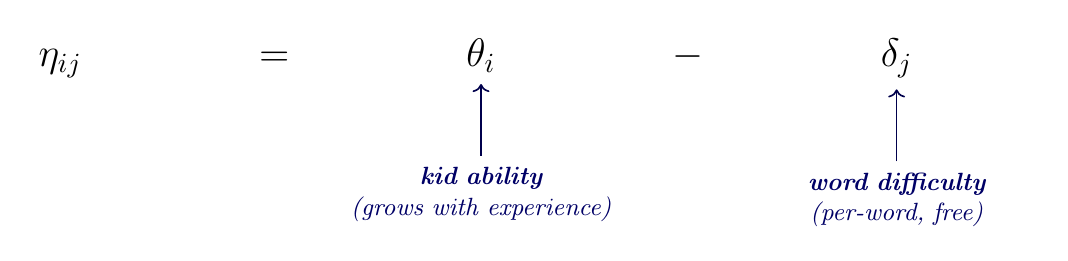
\begin{tikzpicture}[
  every node/.style={inner sep=2pt},
  ann/.style={font=\small\itshape, color=blue!40!black,
              align=center, text width=3.5cm},
  arrow/.style={->, blue!30!black, semithick, shorten >=2pt, shorten <=2pt}]
\matrix[matrix of nodes, column sep=60pt, nodes={font=\Large},
        ampersand replacement=\&]{
  |[name=eta]| $\eta_{ij}$ \&
  $=$ \&
  |[name=theta]| $\theta_i$ \&
  $-$ \&
  |[name=delta]| $\delta_j$ \\
};
\node[ann, below=3em of theta] (atheta)
  {\textbf{kid ability}\\(grows with experience)};
\draw[arrow] (atheta) -- (theta);
\node[ann, below=3em of delta] (adelta)
  {\textbf{word difficulty}\\(per-word, free)};
\draw[arrow] (adelta) -- (delta);
\end{tikzpicture}
\end{document}
